
\فصل{مقدمه}

رمزنگاری مشبکه مبنا شاخه ای از رمزنگاری که مبتی بر پایه مسایل مشبکه می باشد . برتری که این روش در مقایسه با سایر رمزنگاری های مبتی بر نظریه اعداد نظیر تجزیه و لگاریتم گسسته دارد این است که به نظر می آید یک روش پست کوانتوم است و در مقابل کامپیوترهای کوانتومی نمی شکند . در حالی که رمزنگاری مبتنی بر نظریه اعداد شکسته می شود . همچنین معمولا شماهای این رمزنگاری کارایی بالاتر و سرعت بیشتری دارد.  در رمزنگاری مشبکه مبنا، شماهای امن-اثبات پذیر غالبا از توزیع گسسته گوسی استفاده می کنند . الگوریتم ها و روش هایی که برای نمونه برداری از این توزیع وجود دارد ، محاسبات و / یا حافظه نسبتا زیادی می خواهد. با توجه به استفاده و نیاز فراوان به این نمونه برداری قصد داریم هزینه محاسباتی را بهبود دهیم و پیاده سازی سریعی از آن ارایه دهیم. 


رمزنگاری مشبکه مبنا یکی از اصلی ترین انتخاب‌ها برای رمزنگاری پست کوانتوم است . هیچ الگوریتم کوانتوم بهینه‌ای تاکنون نتوانسته است شمای رمز نگاری مشبکه مبنا را بشکند. بر خلاف شماهایی که به طور گسترده در عمل از آنها استفاده می شود همانند RSA  که شکستن آنها بر مبنای سختی شکستن لگاریتم گسسته است ، هم اکنون می توان با استفاده از کامپیوترهای کوانتومی بزرگ شکسته شود. (514) اثبات امن پذیری شمای مشبکه مبنا در گرو عملیات سنگین و سایز بزرگ کلید است . 











\section{نگاشت سراسری}

در نگاشت‌های سراسری همان‌طور که گفته شد، یک تابع مشخص روی تمام پیکسل‌های یک عکس با توجه به متغیرهای عمومی آن اعمال می شود.

\subsection{نگاشت لگاریتمی}
برای محاسبه‌ی تقریبی کدگذاری سیستم بینایی، یک راه حل ساده، استفاده از تابع لگاریتمی است.بنابراین اختلاف واحدها در تصویر با کدگذاری لگاریتمی، نمایشگر اختلاف روشنایی در تصویر است. ایده‌ی اصلی این نگاشت در رابطه ی زیر مشخص شده است. [1] 

در این رابطه$Y$  نشان‌دهنده‌ی روشنایی تصویر، و $D$  نشان‌دهنده‌ی روشنایی دستگاه(صفحه نمایش، چاپگر) است.
میزان روشنایی میانگین تصویر را نیز می‌توان با متغیر $\tau $تغییر داد.

\begin{equation}
Y_{out}  = (D_{max} - D_{min}) \times
 \frac{\log( Y_{in} + \tau) - \log(Y_{min} + \tau)}{\log( Y_{max} + \tau) - \log(Y_{min} + \tau)} 
+ D_{min}
\end{equation}

همان طور که در تصویر مشخسص است ،این نگاشت علی رغم سادگیش، در مقایسه با نگاشت خطی بسیار بهتر عمل  می‌کند.تصویر سمت راست ارائه‌ی عکس با استفاده از نگاشت لگاریتمی، وتصویر سمت چپ، ارائه‌ی همان عکس توسط نگاشت خطی است.
\begin{figure}[!htb]
	\minipage{0.48\textwidth}
	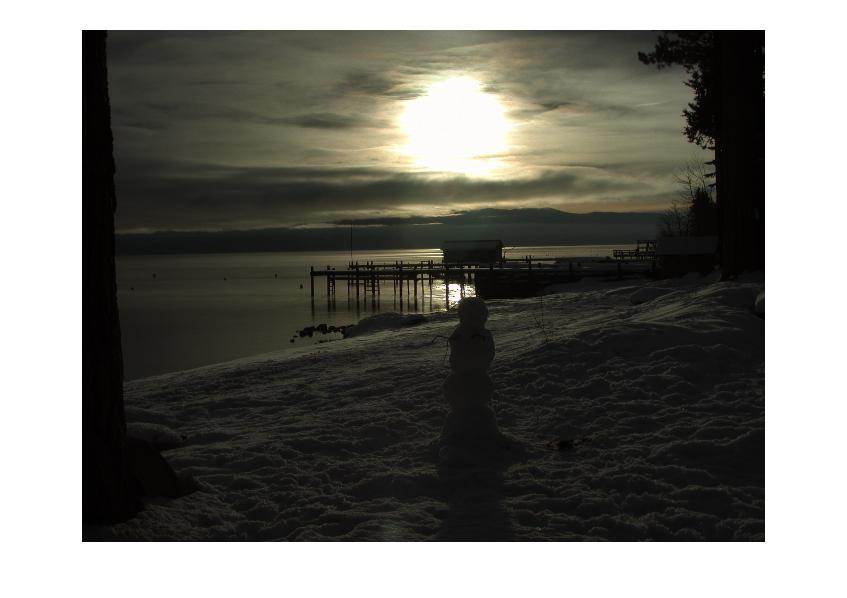
\includegraphics[width=\linewidth]{images/logtonemap}
%	\caption{}\label{fig:logtonemap}
	\endminipage\hfill
	\minipage{0.48\textwidth}
	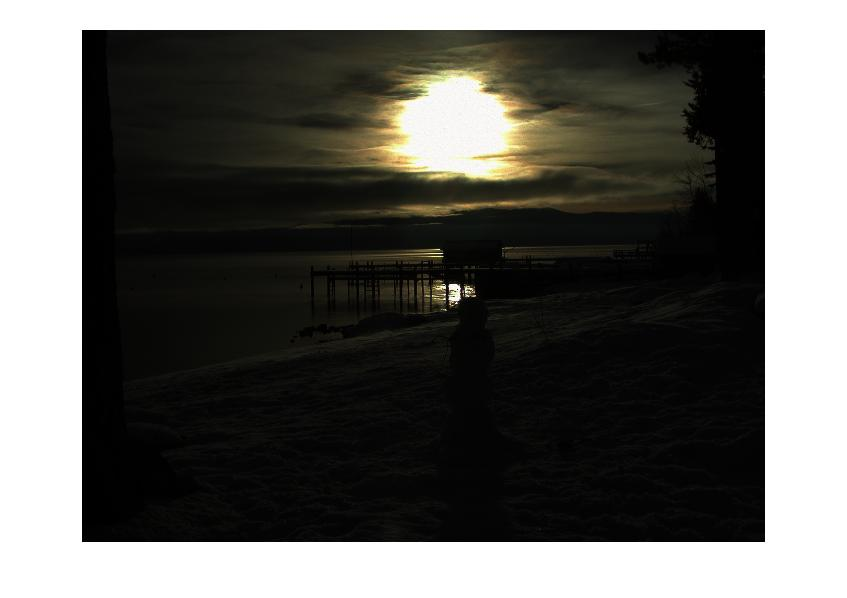
\includegraphics[width=\linewidth]{images/lineartonemap}
	\endminipage\hfill

	\caption{مقایسه‌ی روش‌های
		\متن‌لاتین{tone mapping}: لگاریتمی و خطی
		}\label{fig:linear_vs_log}
\end{figure}

\section{اصلاح نقاط سیاه و سفید}
هر نگاشتی، معمولا شامل این مرحله است که نقاط سیاه عکس را به سیاه، و نقاط سفید تصویر را به سفید نگاشت دهد. در بعضی از نگاشت‌ها مانند نگاشت خطی، این کار خود به خود انجام می‌شود. در غیر این صورت، این کار را پس از نگاشت سراسری انجام می‌دهند تا نتیجه‌ی بهتری بگیرند. در واقع این کار نوعی نگاشت محلی است.

نقاط سیاه و سفید تصویر، به سادگی تیره‌ترین و روشن‌ترین پیکسل‌های تصویر نیستند. زیرا ممکن است به خاطر وجود اختلال، پیکسل‌های پرت داشته باشیم. به همین دلیل، باید گروهی از تیره‌ترین‌ها و گروهی از روشن‌ترین‌ها را پیدا کرد. 
برای این کار می‌توان از روش های هیستوگرام روی 
\متن‌لاتین{luminance image  }
استفاده کرد. به این ترتیب که پیکسل‌های موجود در تصویر را به گروه‌هایی تقسیم کرد که مقدار روشنایی هر گروه، در بازه‌ی مشخصی قرار می گیرد. هر کدام از این بازه ها را 
 \متن‌لاتین{bin  }
 می‌نامیم. 
به این ترتیب، با فرض این که 
 \متن‌لاتین{N}
 تعداد پیکسل‌های موجود در تصویر و 
  \متن‌لاتین{n  }
  تعداد 
  \متن‌لاتین{bin  }
  ها باشد، داریم:

\begin{equation}
N = \sum_{i = 1}^{n} h(i)
\end{equation}
تابع تجمعی 
 \متن‌لاتین{H  }
به شکل زیر تعریف می‌شود، در واقع این تابع نشان دهنده ی مجموع نقاط در بازه های مختلف از 1 تا یک بازه ی خاص 
\متن‌لاتین{j  }
است.:
\begin{equation}
H(j) = \sum_{j^{'} = 1}^{j} h(j^{'})
\end{equation}

\متن‌لاتین{H  }
 یک تابع اکیدا صعودی است. نقاط  سیاه  و سفید 
 \متن‌لاتین{w, b  }
 را به ترتیب نقاطی که در یک درصد ابتدای این تابع قرار می‌گیرند، و نقاطی که در یک درصد آخر قرار می‌گیرند تعریف می‌کنیم.

حال برای اصلاح تصویر، کافی است نقاط سیاه را به 0، نقاط سفید را به 1، و بقیه ی نقاط را به  صورت خطی به  بازه‌ی [0,1]  نگاشت داد. این کار از طریق رابطه ی زیر انجام می شود. قابل ذکر است که طی این تساوی هر کانال رنگ 
\متن‌لاتین{c  }
به بازه ی [0,1] نگاشت می شود.
\begin{equation}
I_{new} = min(1, \frac{max(0, I_{c}(p) - b)}{w - b})
\end{equation}
در تصویر
\ref{fig:bwcorrection}
 یک تصویر سیاه و سفید و در تصویر 
\ref{fig:bwcorrection2}
  یک تصویر رنگی  را قبل و بعد از اصلاح نقاط سیاه و سفید آن مشاهده می کنید.
\begin{figure}[!htb]
 		\minipage{1\textwidth}
 		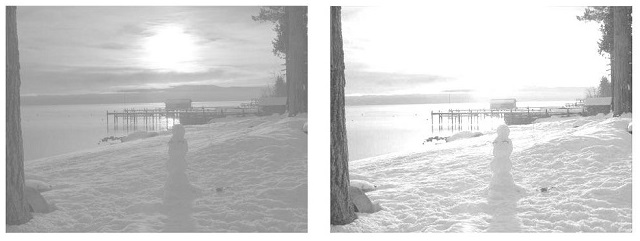
\includegraphics[width=\linewidth]{images/bwcorrection}
 		\caption
 		[حاصل اجرای الگوریتم اصلاح نقاط سیاه و سفید]
 		{
حاصل اجرای الگوریتم اصلاح نقاط سیاه و سفید: عکس سمت راست اصلاح شده‌ی عکس سمت چپ است
}\label{fig:bwcorrection}
 		\endminipage\hfill
 		
 %	\centerline{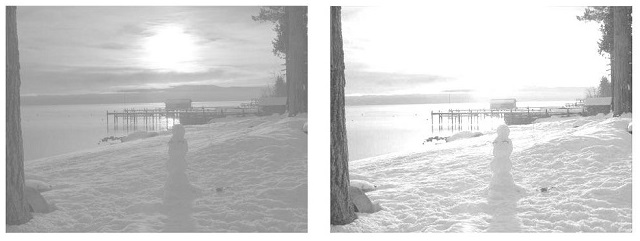
\includegraphics{images/bwcorrection}}
\end{figure}
 \begin{figure}[!tb]
 		\minipage{1\textwidth}
 		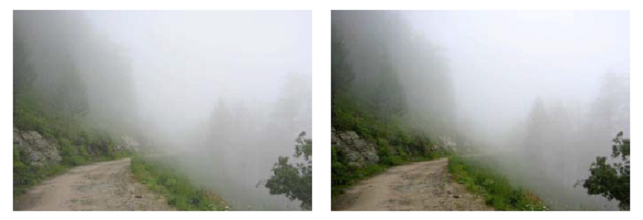
\includegraphics[width=\linewidth]{images/bwcorrection2}
 	\caption
 	[حاصل اجرای الگوریتم اصلاح نقاط سیاه و سفید بر روی عکس رنگی]
{حاصل اجرای الگوریتم اصلاح نقاط سیاه و سفید بر روی عکس رنگی: عکس سمت راست اصلاح شده‌ی عکس سمت چپ است}
 	\label{fig:bwcorrection2}
 	\endminipage\hfill
 %	\centerline{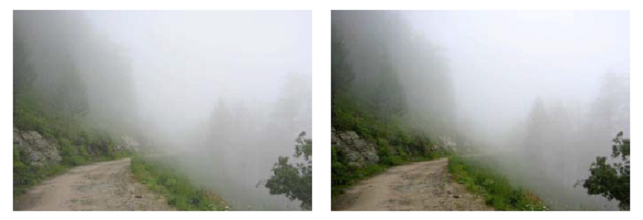
\includegraphics{images/bwcorrection2}}
 \end{figure}